\chapter{Konzeption}
\label{ch:Konzeption3}

Dieses Kapitel beschreibt die Konzeptionsphase eines Prototypen, mit dem der Ansatz dieser Thesis geprüft wird. Hierzu werden in Kapitel \ref{sec:Anwendungsfalle3} Anwendungsfälle  definiert, um anschließend in Kapitel \ref{subsec:Themenfelder3} relevante Themenfelder, zur Implementierung des Prototypen, auf Basis der Anwendungsfälle zu identifizieren. Die identifizierten Themenfelder bilden das technische Konzept zur Umsetzung der Implementierung, die in Kapitel \ref{ch:implementierung4} dargestellt wird.

\section{Definition von Anwendungsfällen}
\label{sec:Anwendungsfalle3}

Dieser Abschnitt erläutert die Wahl der Anwendungsfälle und beantwortet gleichzeitig die erste Teilfrage von \textbf{Forschungsfrage 2} (siehe Kapitel \ref{sec:Zielsetzung1}). Die beiden auserwählten Anwendungsfälle Erkennung von Kreditausfällen und Erkennung von Betrugsversuchen bei Banktransaktionen werden in Kapitel \ref{subsec:Kreditausfallen3} beziehungsweise \ref{subsec:Banktransaktionen3} im Detail erörtert.  

Die Anwendungsfälle wurden anhand der nachfolgenden Kriterien ausgewählt:  

\begin{itemize*}
\item \textbf{Allgemeingültigkeit:} Der Anwendungsfall muss generischer Natur sein, so dass ein entwickeltes Verfahren zur Lösung des Anwendungsfalls in verschiedenen Unternehmen und Branchen angewendet werden kann.      
\item \textbf{Realitätsbezug:} Der Anwendungsfall muss in seiner Komplexität repräsentativ dafür stehen, was auch in realen Softwareentwicklungsprojekten an Komplexität abverlangt wird.     
\item \textbf{Stellenwert des Anwendungsfalls:} Ein möglicher Anwendungsfall muss einen gewissen Stellenwert innerhalb einer Branche besitzen, so dass neue besser funktionierende Verfahren einen messbaren wirtschaftlichen Mehrwert schaffen.
\item \textbf{Automatisierte Entscheidungen:} Kern eines möglichen Anwendungsfalles muss das Treffen einer automatisierten operativen Entscheidung sein. Typischerweise gibt es bereits Lösungen die auf Technologien wie Business Process Management, Business Rules Management oder Decision Management aufsetzen.  
\end{itemize*}

Anhand dieser Kriterien wurden die beiden Anwendungsfälle Erkennung von Kreditausfällen, sowie Erkennung von Betrugsversuchen bei Kreditkartentransaktionen, als am besten geeignet identifiziert. Darüber hinaus wurden auch die Anwendungsfälle Erkennung von Geldwäsche, sowie die Erkennung von Marktmanipulationen evaluiert und als weniger geeignet eingestuft. Die einzelnen Anwendungsfälle werden in den nächsten beiden Unterkapiteln detailliert beschrieben.  

\subsection{Erkennung von Kreditausfällen}
\label{subsec:Kreditausfallen3}

Wie in Kapitel \ref{ch:Motivation1} bereits beschrieben, können Kredite die nicht zurückgezahlt werden zu hohen Verlusten bei Banken führen. Dies wiederum kann zu Finanzkrisen führen, die die komplette Weltbevölkerung in ihren Auswirkungen erreicht. Daher ist die korrekte Erkennung des Kreditrisikos ein elementarer Bestandteil des Kreditvergabeprozesses und maßgeblich verantwortlich für dessen Qualität. 

\begin{figure}[ht]
\centering
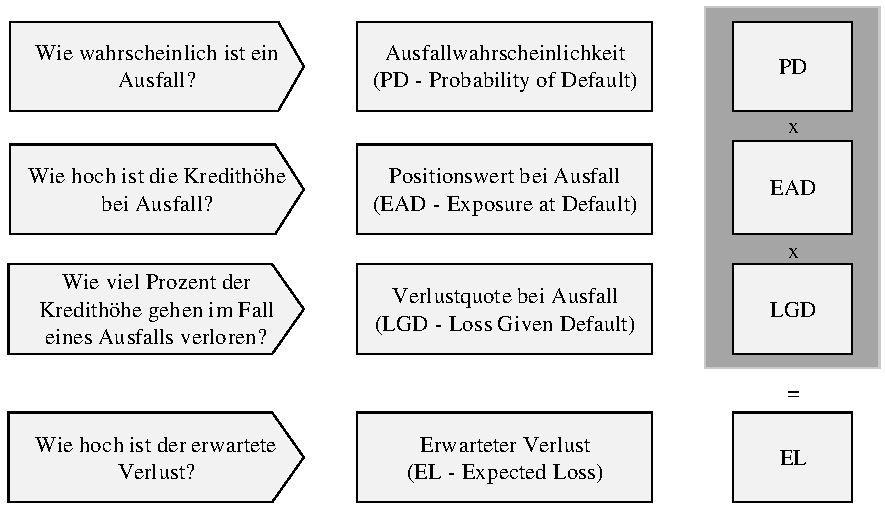
\includegraphics{images/creditriskdimensions.pdf}
\caption{Die Hauptkomponenten des Kreditrisikos.}
\label{fig:creditriskdimensions}
\end{figure}

Die Eigenkapitalvorschrift Basel II ist für alle Banken in Mitgliedsländern der Europäischen Union verpflichtend \cite{RE13} und hält darüber hinaus fest wie Kreditrisiken zu berechnen sind. Abbildung \ref{fig:creditriskdimensions} \cite{GK10} zeigt die Hauptkomponenten zur Berechnung des Kreditrisikos.    

Der erwartete Verlust (EL) bildet die Grundlage zur Bestimmung der Eigenkapitalanforderung an die Bank nach Basel II \cite[vgl. S. 31]{ER11}. Dabei hat das Kreditinstitut die Freiheit Modelle zur Errechnung der Ausfallwahrscheinlichkeit (PD) selbst zu bestimmen, so lange spezifische minimal Anforderungen erfüllt werden. Basel II nennt keine bevorzugte Methode, oder Best-Practice zur Erstellung eines Modells. Engelmann und Rauhmeier nennen die Regressions- und Diskriminanzanalyse als die gängigsten Verfahren zur Modellbildung im Umfeld der Kreditvergabe \cite{ER11}. 

Neben der Berechnung quantitativer Faktoren, fließen auch qualitative Faktoren in die Kreditentscheidung mit ein \cite[vgl. S. 25 ff.]{NB04}. Insbesondere bei Krediten an Firmenkunden besitzt die Betrachtung der qualitativen Faktoren ein hohen Stellenwert. Als Beispiel für mögliche qualitative Faktoren wäre die Branche des Unternehmens, oder die Erfahrung des Managements zu nennen. Im klassischen Privatkunden-Kreditgeschäft, sind komplett automatisierte Bewertungsverfahren die Regel \cite[vgl. S. 31 ff.]{NB04}. Unabhängig vom  Kreditvergabeprozess als Ganzes, muss bei Firmenkunden wie Privatkunden die Ausfallwahrscheinlichkeit ermittelt werden. Diese Thesis wird untersuchen, ob unter der Anwendung von Machine-Learning-Verfahren zur Modellbildung, genauere Vorhersagen erzielt werden können.   

\subsection{Erkennung von Betrugsversuchen bei Banktransaktionen}
\label{subsec:Banktransaktionen3}

Der zweite Anwendungsfall ist das Erkennen von betrügerischen Banktransaktionen. Studien wie \cite{FB11} zeigen, dass durch Kreditkartenbetrug in den Vereinigten Staaten im Jahr 2009, ein Schaden von 190 Milliarden Dollar entstanden ist. Ebenso zeigen Studien \cite[vgl. S. 24]{LE16}, dass im Jahr 2016 66\% aller Betrugsversuche erfolgreich sind. 

Die ACTICO GmbH bietet in ihrer Compliance-Lösung das Modul Name Matching Transaction (NMT) an. Das NMT Modul prüft vor der Ausführung einer Banktransaktion ob ein Betrugsverdacht vorliegt, sollte eine Transaktion als verdächtig eingestuft werden, wird die Ausführung vorübergehend angehalten. In diesem Zeitraum nimmt die Bank Kontakt mit dem Kunden auf und prüft ob die Transaktion so von ihm gewollt war und wieder freigegeben werden darf. 

Eine Transaktion verbindet zwei Parteien, den Auftraggeber der Transaktion und den Empfänger der Transaktion. Sind beide Parteien Kunde der selben Bankinstitution ist keine Prüfung notwendig, da die Transaktion, im Falle eines Betrugs, problemlos widerrufen werden könnte. Sind die beiden Parteien Kunden verschiedener Bankinstitutionen (Entscheidung "`Check fraud relevance"' in Abbildung \ref{fig:fraud-dmn}) beginnt die eigentlich Betrugsprüfung.  

\begin{figure}[ht]
\centering
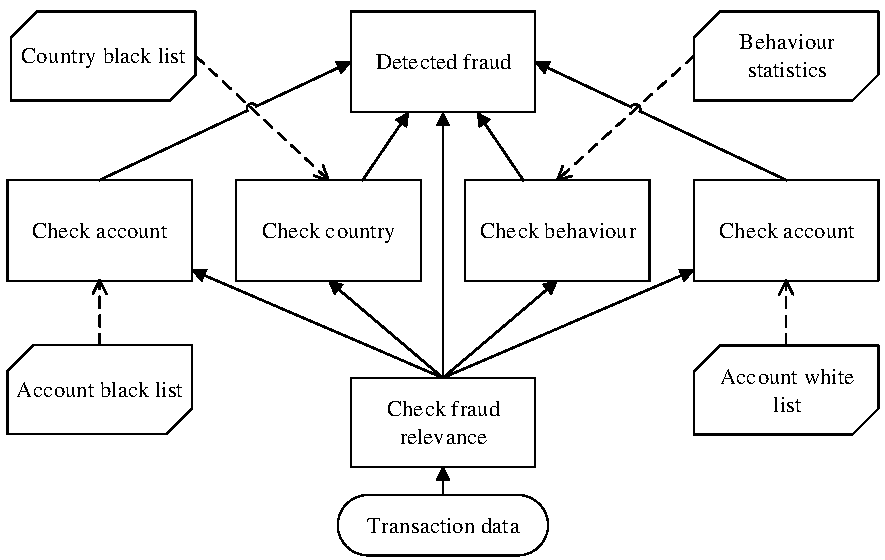
\includegraphics{images/fraud-dmn.pdf}
\caption{Der Transaktionsbetrugsprüfprozess als Decision Requirements Diagram.}
\label{fig:fraud-dmn}
\end{figure}

Die anschließend ausgelöste Betrugsprüfung besteht aus vier Entscheidungen:

\begin{itemize*}
\item \textbf{Account is on black list:} Ein Betrugsfall liegt vor, wenn der Empfänger auf einer "`Black-List"' steht. Derartige Prüflisten werden von öffentlichen Ämtern aber auch von kommerziellen Anbietern veröffentlicht. 
\item \textbf{Target country is on black list:} Ein Betrugsfall liegt vor, wenn das Ziel-Land des Empfängers auf einer Prüfliste steht. 
\item \textbf{Account is on white list:} Ein Betrugsfall liegt nicht vor, wenn der Empfänger auf einer "`White-List"' steht. Eine White-List ist eine Liste mit Bankkonten die als vertrauenswürdig eingestuft wurden. Transaktionen die der Bank-Kunde nachträglich freigeben hat, werden anschließend der White-List hinzugefügt.
\item \textbf{Check behaviour statistics:} Ein Betrugsfall liegt vor, wenn Abweichung in den Nutzungs-Statistiken des Kunden entdeckt wurden. Hierzu zählen ungewöhnliche Zahlungsmethoden, Abweichungen von den üblichen Transaktionszeiten, Abweichungen zu den üblichen Beträgen vorheriger Transaktionen und Abweichungen von der üblichen Menge an Transaktionen in einem Monat. 
\end{itemize*}

Diese Thesis wird untersuchen, ob Machine-Learning-Verfahren besser geeignet sind, anhand der Transaktions-Input-Daten, Betrugsfälle zu erkennen als herkömmliche Ansätze. 

\section{Identifikation relevanter Themenfelder}
\label{subsec:Themenfelder3}

- Klären der Methodik des Prototyping um These zu beweisen

- Erläuterung des Prototypen und dessen Komponenten 
 
GRAFIK PROTOTYPE AT A GLANCE

\subsection{Basisdaten}
\label{subsec:Basisdaten3}

\textbf{Kreditausfall-Erkennung:} Nach ausgiebiger Recherche, konnten über ein Webportal der amerikanischen Hypothekenbank Fannie Mae, geeignete anonymisierte Kreditantragsdaten gefunden werden \cite{FM17}. Alle Datensätze entstammen Einfamilien-Immobilien-Dahrlehn. Die Kreditantragsdatensätze sind über Identifikationsnummern mit Performancedatensätzen verbunden, die das Zahlungsverhalten und weitere Informationen monatlich erfassen \cite{FM18}. Zum Download stehen die Acquisition- (Kreditantragsdaten) und die Performance-Datei (Performancedaten) bereit. Der erste Schritt zur Modellbildung ist die Aufbereitung der Lerndaten, diese bestehen aus Features und einem Label (vgl. \ref{sec:Machine_Learning2}).     
Als Features dienen die Kreditantragsdaten aus der Acquisition-Datei, wobei jeder Kreditantragsdatensatz mehrere Datensätze in der Performance-Datei besitzt. Aus den korrespondierenden Performancedatensätzen, muss für jeden Kreditantragsdatensatz das Label ermittelt werden. Die Kombination aus Features und Label bilden dann den Lerndatensatz. Abbildung \ref{fig:cleansing} soll den Prozess der Lerndatenerzeugung nochmals veranschaulichen.

\begin{figure}[ht]
\centering
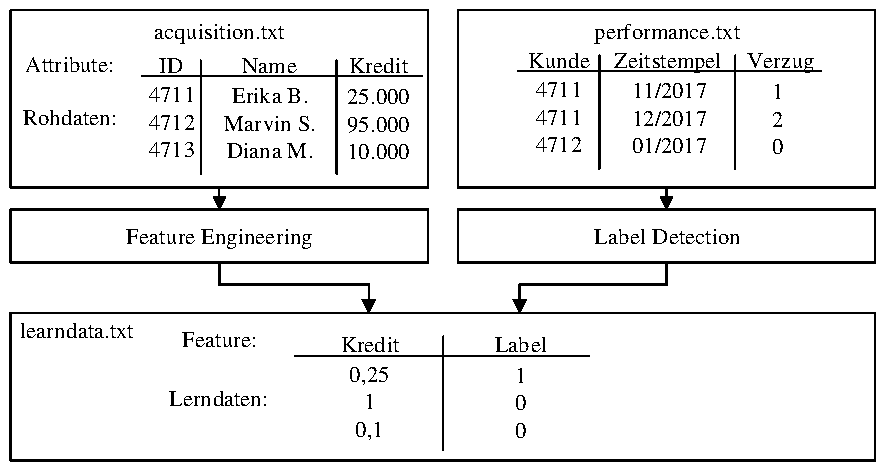
\includegraphics{images/cleansing.pdf}
\caption{Vorgehensweise bei der Erstellung des Lerndatensatzes.}
\label{fig:cleansing}
\end{figure}  

Jeder Datensatz aus der Performance-Datei stellt Informationen über Zahlungsverzüge bereit. Das Feature \textit{Current Loan Delinquency Status} beschreibt wie viele Monate der Kunde in Zahlungsverzug ist. Anhand der Identifikationsnummer wird der aktuellste Datensatz herausgesucht. Befindet sich der Kunde in Zahlungsverzug (Current Loan Delinquency Status > 0), wird dem Label der Wert 1 zu gewiesen. Liegt kein Zahlungsverzug vor wird der Wert 0 zu gewiesen. Darüber hinaus kann Current Loan Delinquency Status auch ''X'' annehmen, wenn der Zahlungsverzug unbekannt ist. Betroffenen Datensätze werden nicht zu Lerndatensätzen umgewandelt und werden übersprungen.  

\subsection{Lerndaten}
\label{subsec:Lerndaten3}

- Welche Daten werden benötigt um unser Neuronales Netz zu füttern.

- Erklärung des Erzeugungs-Algorithmus 

- Erklären von Feature Scaling

- Erklären von Labels

- Grafik mit Beispiel Datensätzen

\subsection{Evaluationsdaten}
\label{subsec:Evaluationsdaten3}

- Welche Daten werden benötigt um unser Neuronales Netz zu evaluieren.

- Erklärung des Erzeugungs-Algorithmus 

- Erklären von Feature Back Scaling

- Grafik mit Beispiel Datensätzen

\subsection{Decision-Engine}
\label{subsec:Engine3}

- Erklärung der theoretischen Funktionsweise der Decision Engine

- Erklärung des Stellenwerts innerhalb des Prototypen

\subsection{Neuronales-Netzwerk}
\label{subsec:Neuro3}
- Erklärung des Stellenwerts innerhalb des Prototypen 

- Funktionale Anforderungen: Lernen können sowie Datensatz evaluieren, sprich Output berechnen können

- Sollte leicht Anpassbar auf verschiedene Daten-Modelle bzw. UseCases sein 

\begin{itemize*}
\item \textbf{PD - Probability of Default:} Die Feststellung der Ausfallwahrscheinlichkeit basierend auf der Bewertung des Kunden, fähig zu sein seinen zukünftigen Zahlungsverpflichtungen nach zu kommen.     
\item \textbf{LGD - Loss Given Default:} Der Verlust bei Ausfall ergibt sich durch die Subtraktion der Sicherheiten von dem Gesamtkreditbetrag. Beispiel: Beträgt die Restschuld eines ausgefallen Kredites 200.000 \euro \hspace{1mm} und der Bank gelingt es die als Sicherheit hinterlegte Eigentumswohnung für 160.000 \euro \hspace{1mm} zu verkaufen, dann beträgt LGD 40.000 \euro.     
\item \textbf{EAD - Exposure at Default:} Abgesehen von wenigen Sonderfällen, beschreibt EAD den restlichen der Bank geschuldeten Betrag zum Zeitpunkt des Ausfalls.
\item \textbf{EL - Expected Loss:} Der erwartete Verlust beschreibt den Wert, den die Bank als Sicherheit in Form von Eigenkapital, nach Basel          
\end{itemize*}